%!TEX root = ../main.tex
\section{Architecture} 
\label{sec:archi}

%To satisfy enterprise customers' needs in the next generation big data solutions, we have designed and implemented \sys, a data lake storage system based on the Huawei OceanStor Pacific storage. The system aims at optimizing the end-to-end processing of massive log messages in big data pipelines. Figure 1 shows the architecture of \sys which consists of store, data service and access three layers from a high-level perspective.

In order to meet the demands of enterprise customers for next-generation big data solutions,  \sys  aims at optimizing the end-to-end processing of massive log messages in big data pipelines. At a high level, \sys is composed of three layers: storage, data service, and data access, as depicted in Figure~\ref{fig:archi}.



 
\begin{figure}[!t]
	\centering
	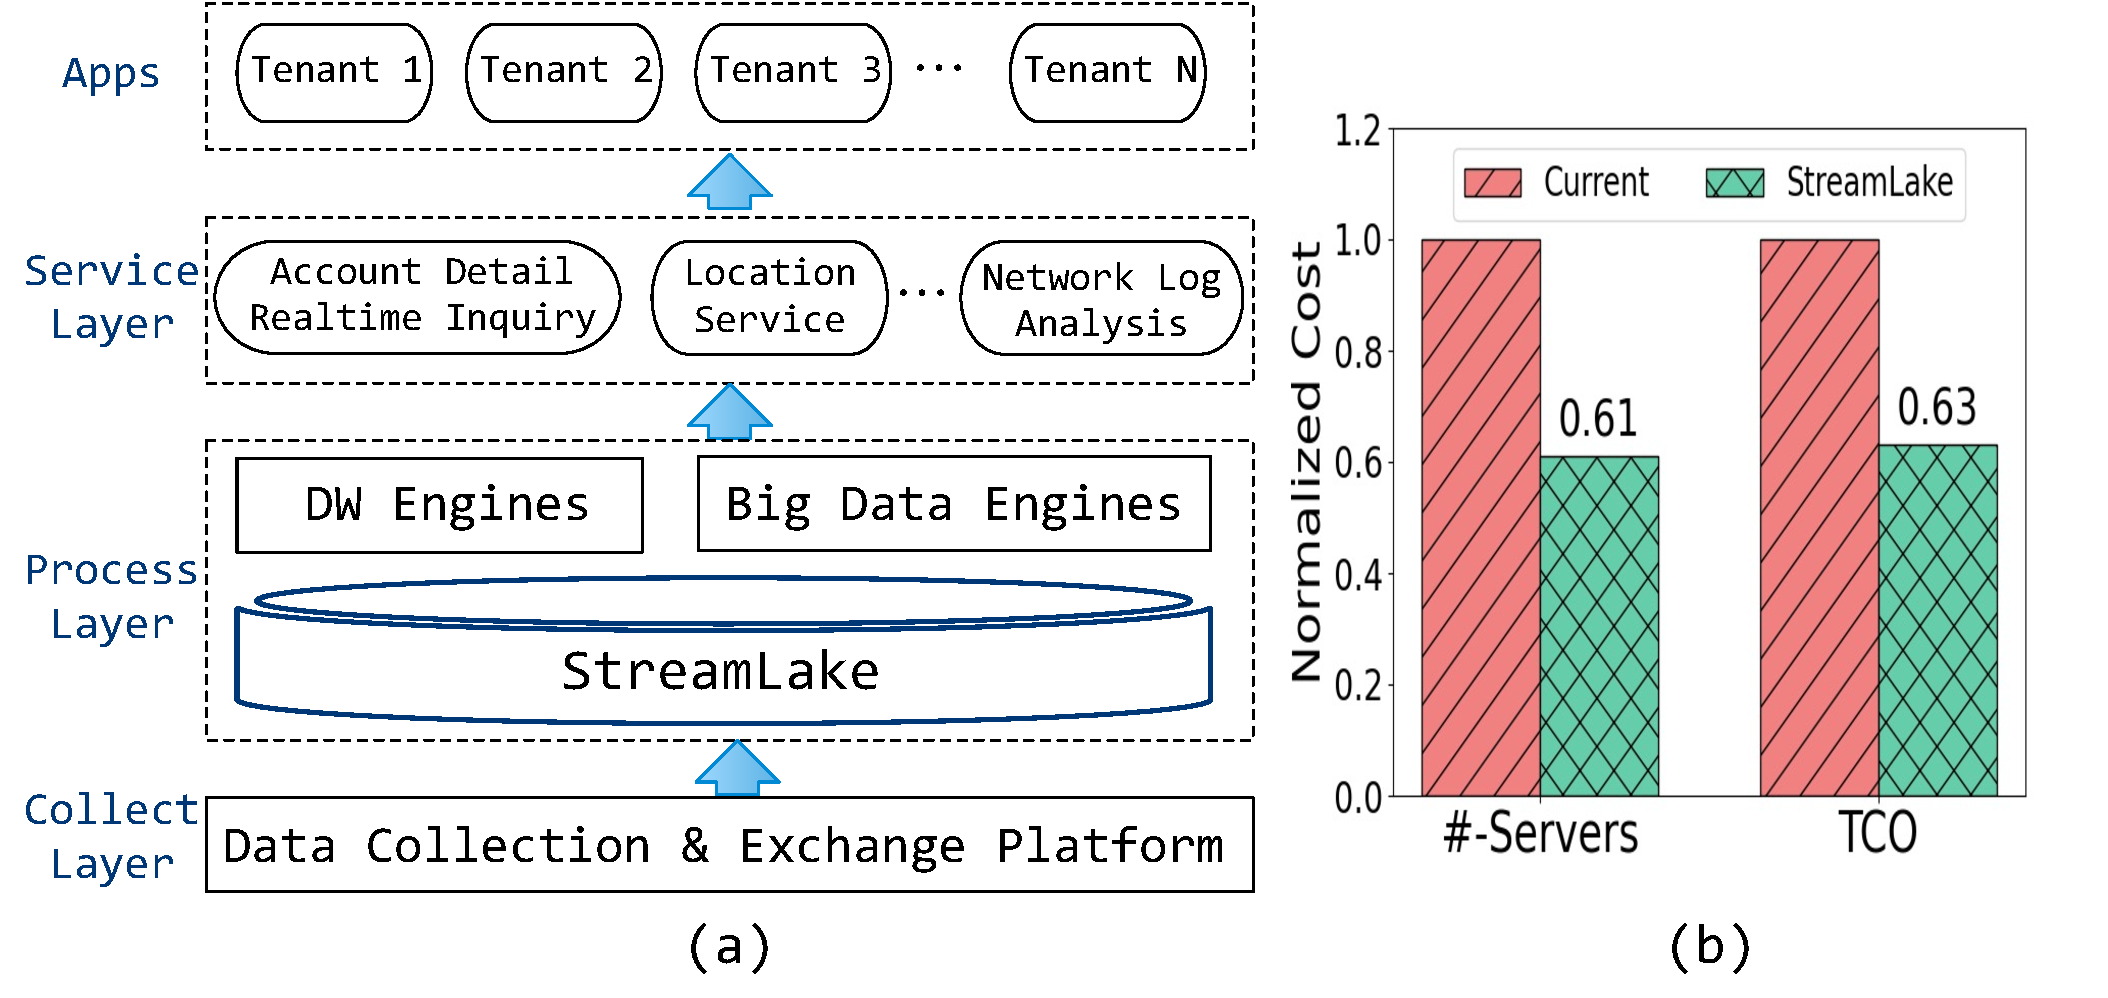
\includegraphics[scale=0.25]{figures/mobile}
	\vspace{-2em}
	\caption{China Mobile Use Case.}
	\label{fig:mobile}
	\vspace{-2em}
\end{figure}

\noindent \textbf{Store layer} is responsible for data persistence, which consists of SSD and HDD data storage pools, a high-speed data exchange and interworking bus as well as multiple types of storage semantic abstractions \cc{(including block, file, stream, table, etc).}


(1) The data storage pools comprised of SSD and HDD offer reliable management of stored data. The physical storage space on the disks in the storage cluster is divided into slices, which are then organized as logical units across various \cc{servers and disks} to ensure data redundancy and load balancing. The storage pools also implement storage space features such as garbage collection, data reconstruction, snapshot, clone, \cc{WORM and thin provision, do we need to talk about this?}, etc. 

%The data storage pools comprised of SSD and HDD offer reliable management of stored data. The physical storage space on the disks in the storage cluster is divided into slices, which are then organized as logical units across various servers and disks to ensure data redundancy and load balancing. Additionally, the storage pools incorporate a range of storage space features such as garbage collection, data reconstruction, snapshot, clone, WORM, and thin provisioning.


(2) \cc{The data exchange and interworking bus} offers high-speed data transfer and interworking of different storage abstractions.Its advanced features include support for Remote Direct Memory Access (RDMA), which bypasses the CPU and L1 cache to accelerate data transfer speeds. Additionally, the bus leverages intelligent stripe aggregation, I/O priority scheduling, and \cc{other state-of-the-art technologies} to optimize data transfer and processing.
All nodes are interconnected by the data bus to enable high  Input/Output Operations per Second (IOPS), large bandwidth and low latency data exchanges. Furthermore, the bus supports the interworking of different storage abstractions, allowing for the sharing and  access of a single data piece by different interfaces, which eliminates the need for data migration and significantly saves storage space.

(3) The block, file and \cc{other storage abstraction} implement access interfaces to the underlying storage in different semantics. We introduce two new abstractions, stream object and table object, to manage messaging streams and tabular data efficiently. 
Their implementation will be discussed in Section~\ref{sec:datagen}.


\noindent \textbf{Data service layer} provides a rich set of features to enable efficient data management at enterprise scale. For instance, the tiering service offers static and dynamic data migration and eviction between the SSD and HDD storage pools based on tiering policies, which saves the storage cost a lot. The replication service provides periodical replications to remote sites for backup and recovery. Particularly, to further enhance the capabilities of the layer, we have extended it to include specialized services and optimizations for log message processing operations, which include the \sys  services (Section~\ref{sec:dataeva}) to support \cc{real-time streaming and lakehouse functionality}, and \brain (Section~\ref{sec:lakebrain}) to improve the resource utilization and query efficiency.
 
 \cc{Not specific enough:above, how to involve Elastic Serverless Function Engine? }

% These services and optimizations are elaborated in section 5 and 6.
% The elastic serverless function engine is a component that we introduce to support near data processing of the StreamLake services. Its design is discussed in section 5.3. 

%To further enhance the capabilities of the Data Service Layer, we have extended it to include specialized services and optimizations for log message processing operations. These include the StreamLake services and LakeBrain optimization, which are elaborated in Sections 5 and 6 of our report.

%To support near-data processing of the StreamLake services, we have introduced a new component called the Elastic Serverless Function Engine. Its design and functionality are discussed in detail in Section 5.3.


\noindent \textbf{Data access layer} implements storage access protocols to handle user requests. It supports a block service via standard iSCSI access, NAS services via NFS and SMB protocols as well as an object service via S3 protocol, etc.
The new StreamLake services utilize the OceanStor distributed Parallel Client (DPC) which is a universal protocol-agnostic client providing shorter but superfast IO path. 
 %The new StreamLake services utilize the OceanStor distributed Parallel Client (DPC), a universal protocol-agnostic client that provides a shorter but super-fast IO path.
The Access Layer also plays a crucial role in managing authentication and \cc{ACL} permission control, which ensures that only valid user requests are translated into internal requests for further processing, so as to achieve  the security and integrity.
 
 

 
 
 
 
 \begin{figure}[!t]
 	\centering
 	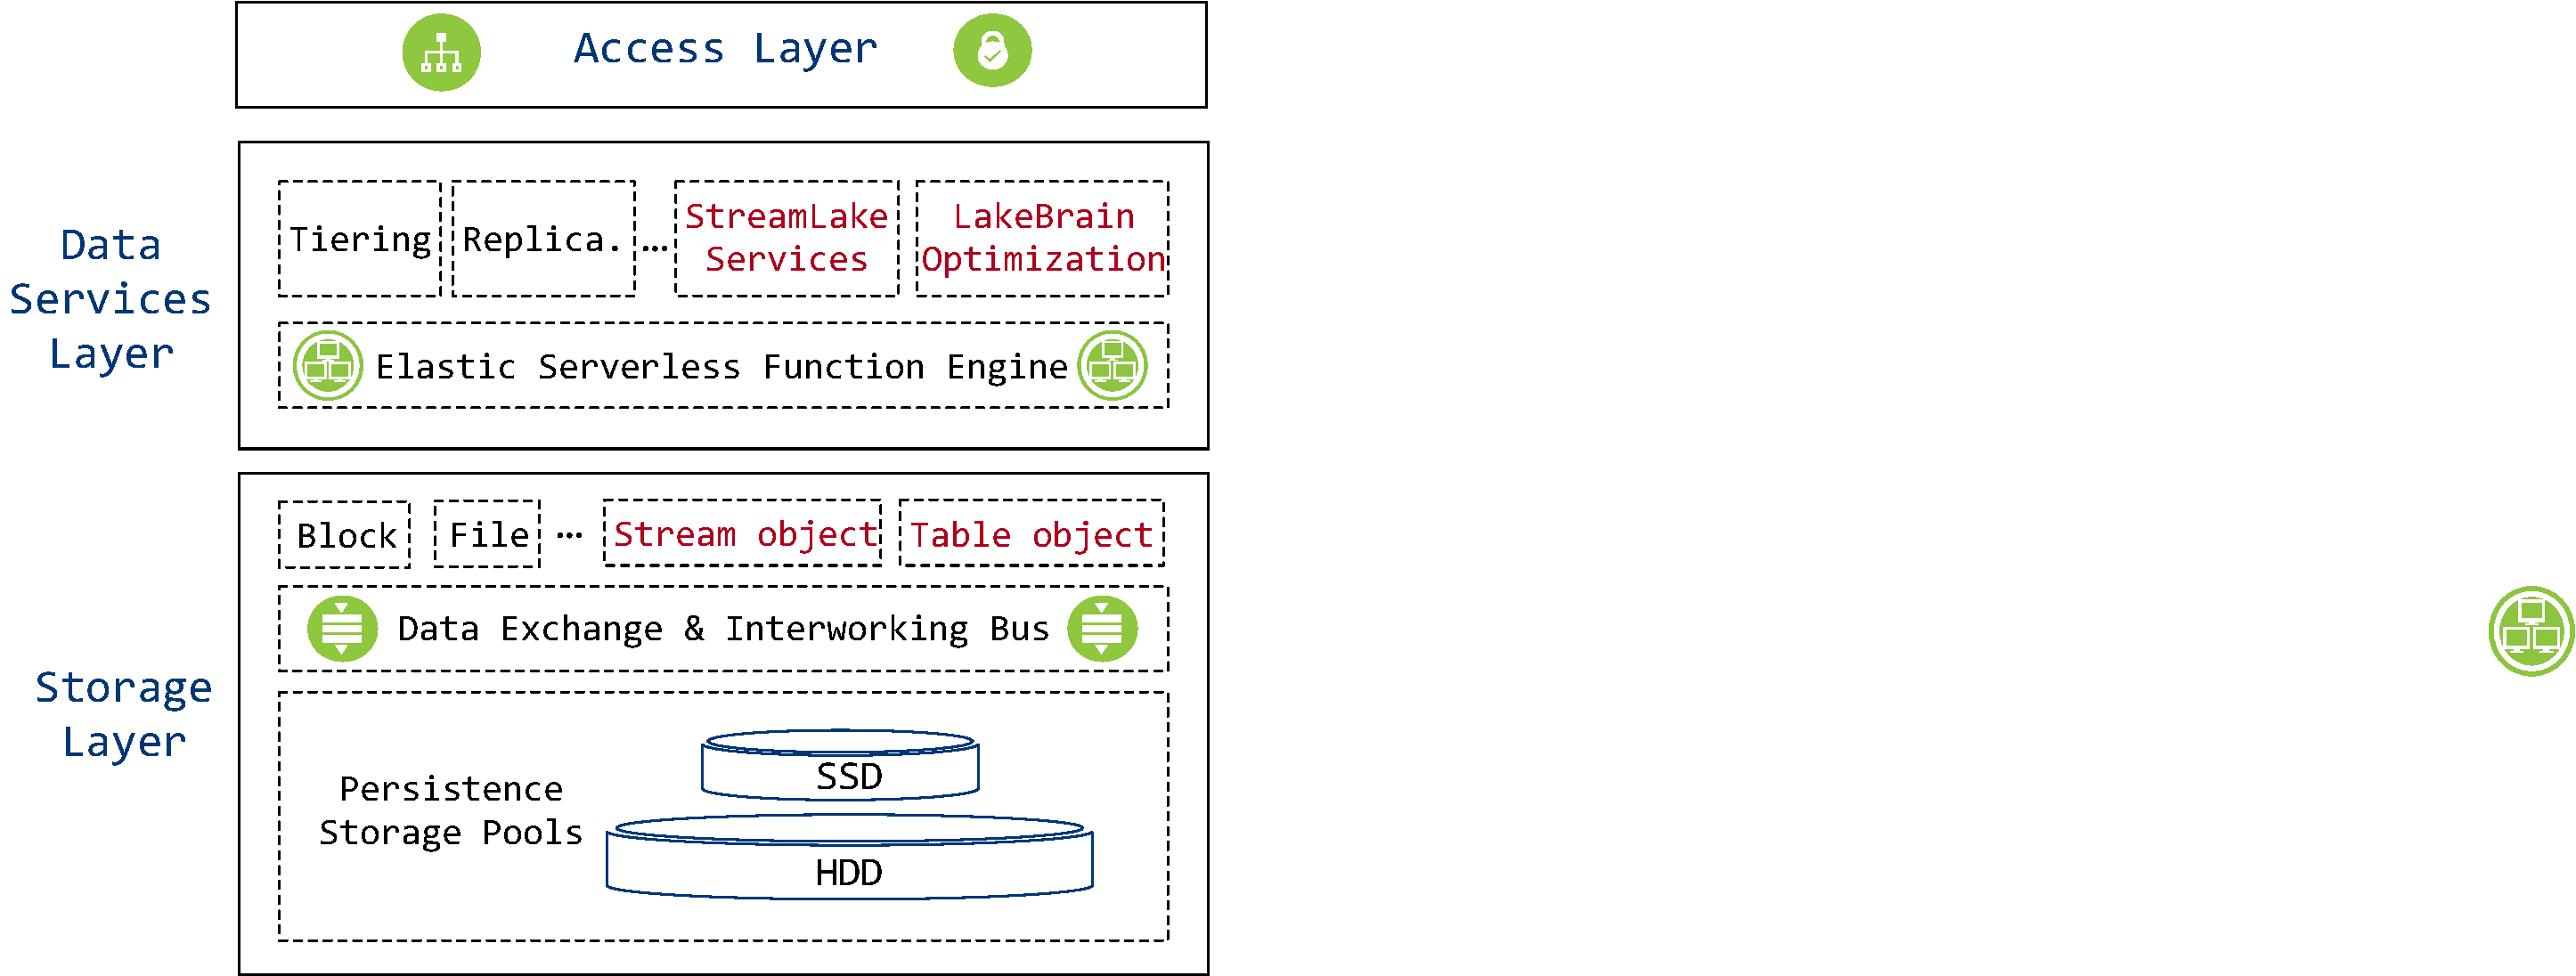
\includegraphics[scale=0.35]{figures/archi}
 	\vspace{-1em}
 	\caption{\sys Storage Architecture.}
 	\label{fig:archi}
 	\vspace{-2em}
 \end{figure}
 
 
 